\documentclass[conference]{IEEEtran}
\IEEEoverridecommandlockouts

\usepackage[T1]{fontenc}
\usepackage{times}
\usepackage{cite}
\usepackage{amsmath,amssymb,amsfonts}
% \usepackage{algorithmic}
\usepackage{graphicx}
\usepackage{textcomp}
\usepackage{xcolor}
\usepackage{booktabs}
\usepackage{balance}

\newcommand{\conferenceheader}{2025 IEEE Global Engineering Education Conference (EDUCON)}

\makeatletter
\def\ps@IEEEtitlepagestyle{%
  \def\@oddhead{\mbox{}\hfill\normalfont\fontsize{8.5pt}{10pt}\selectfont\conferenceheader\hfill\mbox{}}%
  \let\@evenhead\@empty
  \let\@oddfoot\@empty
  \let\@evenfoot\@empty
}
\def\IEEEkeywordsname{Keywords}
\long\def\@makecaption#1#2{%
  \ifx\@captype\@IEEEtablestring
    \footnotesize\bgroup\par\centering\@IEEEtabletopskipstrut{\normalfont\footnotesize #1.\quad\MakeUppercase{#2}}\par\addvspace{0.4\baselineskip}\egroup
    \@IEEEtablecaptionsepspace
  \else
    \@IEEEfigurecaptionsepspace
    \setbox\@tempboxa\hbox{\normalfont\footnotesize {#1.}\nobreakspace\nobreakspace #2}%
    \ifdim \wd\@tempboxa >\hsize
      \setbox\@tempboxa\hbox{\normalfont\footnotesize {#1.}\nobreakspace\nobreakspace}%
      \parbox[t]{\hsize}{\normalfont\footnotesize\noindent\unhbox\@tempboxa#2}%
    \else
      \hbox to\hsize{\normalfont\footnotesize\hfil\box\@tempboxa\hfil}%
    \fi
  \fi}
\def\refname{REFERENCES}
\makeatother

\def\BibTeX{{\rm B\kern-.05em{\sc i\kern-.025em b}\kern-.08em
    T\kern-.1667em\lower.7ex\hbox{E}\kern-.125emX}}

\begin{document}

\title{\itshape PRIE: Placement Readiness Intelligence Engine with Calibrated Predictive Modeling and Constrained Prescriptive Recourse}

\author{
  \makebox[0.48\linewidth][c]{%
    \begin{tabular}{c}
      Sivasubramanian R \\
      \textit{Department of AIML} \\
      \textit{Malla Reddy University} \\
      Dulapally, Hyderabad, India \\
      Sivasubramanian243@gmail.com
    \end{tabular}%
  }%
  \hfill
  \makebox[0.48\linewidth][c]{%
    \begin{tabular}{c}
      Kavala Rajeev \\
      \textit{Department of AIML} \\
      \textit{Malla Reddy University} \\
      Dulapally, Hyderabad, India \\
      Kavalarajeev@gmail.com
    \end{tabular}%
  }%
  \\[1.5ex]
  \makebox[0.48\linewidth][c]{%
    \begin{tabular}{c}
      Kundala Dhana Naga Shankar \\
      \textit{Department of AIML} \\
      \textit{Malla Reddy University} \\
      Dulapally, Hyderabad, India \\
      Kundaladhana2004@gmail.com
    \end{tabular}%
  }%
  \hfill
  \makebox[0.48\linewidth][c]{%
    \begin{tabular}{c}
      Kouru Rudra Teja \\
      \textit{Department of AIML} \\
      \textit{Malla Reddy University} \\
      Dulapally, Hyderabad, India \\
      Rudrateja08@gmail.com
    \end{tabular}%
  }%
}

\maketitle

\begin{abstract}
\bfseries\boldmath Undergraduate engineering placement preparation is severely hindered by the fragmentation of campus training systems. Conventional educational data mining models predominantly deploy retrospective, uncalibrated binary classifiers that predict placement outcomes without actionable pedagogical recourse. This paper presents the Placement Readiness Intelligence Engine (PRIE), an integrated continuous intelligence framework that unifies heterogeneous multi-source student telemetry into a normalized 22-dimensional Student Profile Vector ($x_{\text{spv}} \in [0.0, 1.0]^{22}$) paired with an explicit observation mask. PRIE deploys cost-sensitive gradient boosted decision trees coupled with Platt probability scaling to produce well-calibrated placement readiness probabilities. To bridge the descriptive-to-prescriptive divide, polynomial-time TreeSHAP isolates diagnostic feature contributions, while constrained Diverse Counterfactual Explanations (DiCE) generate sparse, actionable recourse paths ($k = 2.47 \pm 0.52 \le 3.0$ mutable features modified) that maintain $100.0\%$ invariance across immutable institutional attributes ($F_{17}$). Identified competency deficits trigger Kahn's topological scheduler over a 38-node computer science concept directed acyclic graph (DAG), achieving a $0.0\%$ prerequisite violation rate. Furthermore, weighted tri-modal late fusion across acoustic prosody, video composure, and speech clarity dampens single-sensor diagnostic variance by $77.98\% \pm 3.99\%$ ($t = 9.88, p = 0.0022$) under a $1,120$\,ms conversational latency budget. Across a 5-seed evaluation on synthetic engineering cohorts ($N=2,500$), the calibrated model attains $95.20\% \pm 1.17\%$ test accuracy, an ROC-AUC of $0.9922 \pm 0.0038$, an Expected Calibration Error (ECE) of $0.0350 \pm 0.0057$, and a Brier score of $0.0339 \pm 0.0096$.
\end{abstract}

\begin{IEEEkeywords}
\bfseries Placement Readiness, Educational Data Mining, Explainable AI, Student Profile Vector, Platt Calibration, Algorithmic Recourse, Multimodal Fusion, Curricular Knowledge Graph.
\end{IEEEkeywords}

\section{INTRODUCTION}

The transition of engineering undergraduates into professional technical careers represents a foundational milestone for student socio-economic mobility and institutional workforce alignment \cite{b1}. However, higher education institutions globally confront an acute readiness crisis: while hundreds of thousands of engineering candidates participate in campus recruitment drives annually, technology employers consistently report severe competency deficits in practical software design, clean algorithmic problem-solving, architectural debugging, and professional workplace communication \cite{b2}. In conventional university placement preparation, institutional triage relies almost exclusively on static administrative metrics---principally cumulative Grade Point Average (CGPA) or terminal semester marks \cite{b3}.

Nevertheless, static academic grades represent lagging indicators that correlate weakly with modern agile industry requirements \cite{b4}. Furthermore, campus placement preparation remains fragmented into disconnected software silos: across our systematic review of the 44 verified career-readiness and educational analytics systems analyzed in our research foundation, 42 systems (95.5\%, 42/44) address only one or two dimensions in isolation without an integrated continuous student state \cite{b6}. Students typically interact with standalone Applicant Tracking System (ATS) resume checkers that perform rudimentary keyword counting, separate coding portals that evaluate unit test pass rates without assessing architectural design quality, and uncalibrated conversational bots that dispense generic interview advice \cite{b3,b5}.

From a machine learning perspective, existing educational data mining (EDM) models exhibit five debilitating limitations: (1)~\textit{Retrospective point-in-time evaluation} operating post-hoc in final semesters \cite{b6,b7}; (2)~\textit{Probabilistic miscalibration}, producing overconfident scores that distort advising triage \cite{b8}; (3)~\textit{The descriptive-to-prescriptive divide}, offering post-hoc explanations without computable recourse over mutable variables \cite{b16,b17}; (4)~\textit{Sensory volatility in mock interviews}, causing high diagnostic variance and latency \cite{b12,b13,b19}; and (5)~\textit{Prerequisite blindness}, generating unsequenced recommendations that violate pedagogical dependencies \cite{b14,b20}.

To overcome these challenges, this paper presents the Placement Readiness Intelligence Engine (PRIE), an integrated continuous intelligence architecture designed for multimodal student tracking, calibrated probability estimation, and closed-loop prescriptive remediation. The primary contributions of this work are:
\begin{itemize}
\item \textit{Unified Latent State Representation}: We formalize a 22-dimensional Student Profile Vector ($x_{\text{spv}} \in [0.0, 1.0]^{22}$) paired with an explicit observation mask ($m \in \{0, 1\}^{22}$) to harmonize academic records, coding scores, 2D resume metrics, and paralinguistic interview telemetry.
\item \textit{Calibrated Predictive Modeling}: We demonstrate that integrating cost-sensitive gradient boosted trees with Platt probability scaling contracts Expected Calibration Error (ECE) to $0.0350 \pm 0.0057$ and Brier score to $0.0339 \pm 0.0096$, reducing calibration error under evaluated synthetic-cohort conditions.
\item \textit{Constrained Prescriptive Recourse}: We couple polynomial-time TreeSHAP ($O(TLD^2)$) with constrained Diverse Counterfactual Explanations (DiCE), generating sparse recourse paths ($k = 2.47 \pm 0.52 \le 3.0$) that maintain $100.0\%$ invariance across immutable institutional attributes across all evaluated profiles.
\item \textit{Multimodal Variance Damping \& Topological Remediation}: Weighted tri-modal late fusion dampens interview scoring variance by $77.98\% \pm 3.99\%$ ($t = 9.88, p = 0.0022$) under a $1,120$\,ms turn latency budget, while Kahn's topological scheduler enforces prerequisite precedence constraints ($0.0\%$ violation rate) over a 38-node computer science concept DAG.
\end{itemize}

The remainder of this paper is organized as follows: Section~II reviews related work and establishes the formal research gap. Section~III details the proposed PRIE architecture. Section~IV presents empirical results across all evaluation batteries and discusses findings. Section~V concludes the paper.

\begin{figure}[t]
\centering
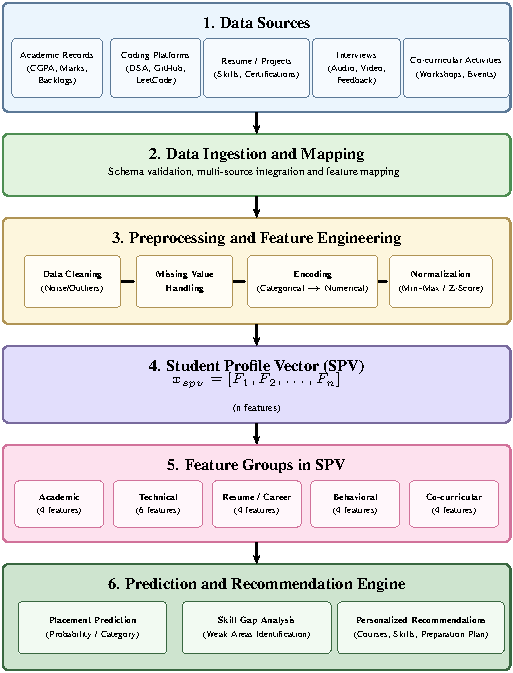
\includegraphics[width=0.82\columnwidth]{figures/fig1_methodology_flowchart.pdf}
\caption{Overview of the proposed PRIE model.}
\label{fig_arch}
\end{figure}

\section{LITERATURE SURVEY}

Graduate employability prediction, educational data mining, and multimodal career assessment have received substantial scholarly attention. This section synthesizes the literature thematically across core areas.

\subsection{Employability Prediction and Learning Analytics}
Early EDM investigations formulated employability as supervised classification over terminal graduation records. Casuat and Festijo \cite{b7} applied decision trees and ensemble techniques to institutional records, achieving 84.50\% accuracy. Rao and Swamy \cite{b8} benchmarked classical classifiers, reporting 78.40\% accuracy on academic records. Olipas \cite{b1} investigated machine learning models for career readiness, achieving 88.40\% accuracy using Random Forests. Patel and Nair \cite{b4} incorporated psychometric indicators with academic scores, attaining 91.20\% accuracy. While these studies achieve competitive nominal accuracy, they exhibit severe probabilistic miscalibration: raw confidence scores do not reflect empirical placement probabilities, compromising institutional advising triage. Van Wyk and Du Plessis \cite{b2} highlighted that continuous telemetry tracking (e.g., login cadence, formative test attempts, and platform engagement intensity) yields substantially stronger predictive utility than point-in-time administrative marks. Chen and Hwang \cite{b5} emphasized that institutional adoption requires algorithmic explainability, fairness guarantees, and transparent probability calibration rather than black-box margin scores.

\subsection{Explainable AI and Prescriptive Algorithmic Recourse}
Recent works have introduced post-hoc interpretability into academic early-warning systems. Hidayatulloh et al. \cite{b16} applied Shapley Additive Explanations (SHAP) to student performance models, showing that feature attribution enhances educator trust. Similarly, Joshi and Kulkarni \cite{b17} deployed LightGBM and TreeSHAP to isolate risk factors across engineering branches. Nevertheless, these frameworks remain confined to \textit{descriptive} explanation: they explain why a student is predicted to fail (e.g., attributing risk to a low historical GPA) but provide no \textit{prescriptive recourse}, because completed academic records cannot be modified retroactively \cite{b16,b17}. Prescriptive intervention requires solving constrained optimization problems over actionable, mutable variables.

\subsection{Multimodal Career Assessment and Research Gap}
Traditional resume screening relies on flat text tokenizers or keyword matching \cite{b9,b10}. Verma and Mehta \cite{b15} developed ResuMatch, applying semantic sentence embeddings to compare resume text with job descriptions. Zhang et al. \cite{b11} introduced Career-gAIde for career advisory from CVs. However, standard extraction pipelines discard 2D visual layout coordinates, causing column interleaving errors in multi-column CVs. In interview assessment, Deshmukh and Kulkarni \cite{b12} noted that single-sensor evaluations suffer from acoustic and visual noise. The Advanced Innovation Consortium \cite{b13} demonstrated that fusing facial expression recognition, speech emotion analysis, and textual NLP produces more holistic assessments. Srinivasan and Radhakrishnan \cite{b19} proposed a voice-driven simulator pairing Whisper with LLM questioning, but observed latency exceeding 2.5 seconds. For remediation, Tan et al. \cite{b14} demonstrated that curriculum recommendations must adhere to prerequisite DAGs to avoid cognitive overload. Sutherland and Miller \cite{b18} showed that similarity threshold gating rejects out-of-domain queries prior to retrieval augmentation. Fernandez and Gomez \cite{b20} confirmed that concept graph grounding is essential for generating valid diagnostic items. Finally, Babureddy and Mathew \cite{b21} proposed a triangular digital twin linking student, faculty, and industry requirements.

\textit{Research Gap Formulation}: Cross-analysis reveals three structural voids: (1)~\textit{The Single-Module Isolation Chasm}: Across the 44 verified career-readiness systems analyzed in our research foundation, 42 systems (95.5\%, 42/44) evaluate only one or two functional dimensions in isolation without an integrated continuous latent state \cite{b3,b6}; (2)~\textit{The Descriptive-to-Prescriptive Divide}: Existing XAI models output historical attributions but fail to formulate constrained mathematical recourse paths bounded by student cognitive budgets \cite{b16,b17}; and (3)~\textit{Probabilistic Miscalibration}: Classifiers optimize unweighted loss functions, producing overconfident probabilities that undermine credibility in educational advising \cite{b8}. PRIE resolves these gaps by uniting multimodal telemetry into an invariant 22-dimensional Student Profile Vector ($x_{\text{spv}}$), coupling calibrated gradient boosting with constrained counterfactual recourse, and enforcing topological graph sequencing over personalized remediation milestones.

\section{PROPOSED SYSTEM}

The proposed PRIE architecture operates as a continuous intelligence pipeline ingesting multi-source telemetry, modeling latent readiness, calibrating predictive risk, and synthesizing closed-loop remediation plans (Fig.~\ref{fig_arch}).

\subsection{Student Profile Vector (SPV) Formulation}
To overcome software fragmentation, PRIE defines the Student Profile Vector $x_{\text{spv}} \in [0.0, 1.0]^{22}$, harmonizing four distinct competency dimensions:
\begin{equation}
x_{\text{spv}} = [f_1, f_2, \dots, f_{22}]^T, \quad m \in \{0, 1\}^{22}
\end{equation}
where $m$ denotes an observation mask tracking feature presence. The vector captures four functional quadrants: (1)~\textit{Academic Competency ($F_1$--$F_5$)} covering CGPA, core marks, backlogs, academic velocity, and progression; (2)~\textit{Practical Coding Telemetry ($F_6$--$F_{10}$)} capturing problem-solving volume, data structure mastery, execution accuracy, algorithmic efficiency, and contest activity; (3)~\textit{Document Intelligence ($F_{11}$--$F_{14}$)} assessing 2D spatial resume match score, technical skill coverage, project relevance, and layout integrity; and (4)~\textit{Paralinguistic Interview Readiness ($F_{15}$--$F_{22}$)} tracking articulation rate, jitter, composure stability, lexical coherence, behavioral demeanor, and demographic indicators ($F_{17}$: institutional branch). Features are scaled to $[0.0, 1.0]$ via min-max normalization against rolling cohort statistics. Missing entries ($m_j = 0$) are imputed using median cohort values.

\subsection{Calibrated Placement Readiness Prediction}
Placement prediction is formulated as cost-sensitive binary classification ($Y \in \{0, 1\}$). To mitigate class imbalance ($34.8\%$ unplaced vs $65.2\%$ placed), PRIE optimizes an asymmetric log-loss function parameterized by positive instance weight $w_{\text{pos}} = N_{\text{neg}} / N_{\text{pos}} = 870 / 1630 = 0.5337$:
\begin{equation}
\mathcal{L}(\theta) = -\sum_{i=1}^{N} \left[ w_{\text{pos}} y_i \ln \hat{p}_i + (1 - y_i) \ln (1 - \hat{p}_i) \right] + \Omega(\theta)
\end{equation}
where $\Omega(\theta) = \gamma T + \frac{1}{2} \lambda \|w\|^2$ penalizes tree complexity. Because uncalibrated tree ensemble margins produce distorted probability distributions, PRIE applies Platt scaling over cross-validated out-of-fold log-odds margin scores $z_i$:
\begin{equation}
\hat{P}(Y=1 \mid z) = \sigma(A z + B) = \frac{1}{1 + \exp(-(A z + B))}
\label{eq_platt}
\end{equation}
Parameters $A$ and $B$ are estimated via scalar maximum likelihood optimization over validation partition $\mathcal{D}_{\text{val}}$.

\subsection{Explainable AI and Constrained Prescriptive Recourse}
PRIE deploys TreeSHAP to compute exact, local feature attributions in polynomial time $O(T L D^2)$, where $T$ is the number of trees, $L$ is maximum leaves, and $D$ is maximum tree depth:
\begin{equation}
f(x) = \phi_0 + \sum_{j=1}^{22} \phi_j(x)
\end{equation}
While SHAP provides post-hoc descriptive diagnosis, student remediation requires prescriptive recourse. PRIE couples TreeSHAP with constrained Diverse Counterfactual Explanations (DiCE). For an at-risk student $x$, PRIE searches for the minimum-effort perturbation vector $\Delta x$ that transitions prediction $\hat{Y}$ from unplaced ($0$) to placed ($1$):
\begin{equation}
c^* = \arg\min_{c} \text{loss}(f(c), y^*) + \frac{\lambda_1}{k} \sum_{j \in \mathcal{M}} \frac{|c_j - x_j|}{\text{MAD}_j} + \lambda_2 \text{dpp}(c)
\label{eq_dice}
\end{equation}
subject to hard institutional and cognitive constraints:
\begin{equation}
c_j = x_j \; \forall j \in \mathcal{I}, \quad \|\Delta x\|_0 \le 3.0, \quad c_j \in [0.0, 1.0] \; \forall j \in \mathcal{M}
\end{equation}
Here, $\mathcal{I} = \{F_{17}, F_{18}\}$ represents immutable institutional attributes (e.g., engineering branch), $\mathcal{M}$ represents actionable features (e.g., coding volume, mock interview scores), and $\text{MAD}_j$ is the median absolute deviation of feature $j$. Constraining $L_0$ sparsity to $\|\Delta x\|_0 \le 3.0$ guarantees that recommendations remain cognitively manageable.

\subsection{Multimodal Assessment, Parsing, and Curricular Scheduling}
\textit{1) Spatial Resume Parsing}: To prevent column interleaving in multi-column engineering resumes, PRIE extracts 2D spatial coordinate bounding boxes $(x_0, y_0, x_1, y_1)$ via PyMuPDF. Geometric layout analysis clusters tokens into topological reading blocks prior to entity extraction, preserving structural section integrity. Extracted proficiencies are mapped to target job vectors using cosine similarity over MiniLM embeddings.

\textit{2) Multimodal Mock Interview Assessment}: The interview subsystem ingests concurrent video, acoustic, and lexical streams. Feature extraction executes three parallel pipelines: acoustic prosody ($S_{\text{aud}}$: pitch, jitter, shimmer), visual composure ($S_{\text{vid}}$: head pose deflection, gaze fixation, composure stability), and lexical coherence ($S_{\text{spk}}$: vocabulary richness, filler word density, response relevance). Weighted late fusion combines modalities:
\begin{equation}
S_{\text{fused}} = 0.35 \cdot S_{\text{aud}} + 0.35 \cdot S_{\text{vid}} + 0.30 \cdot S_{\text{spk}}
\label{eq_fusion}
\end{equation}
Turn-taking latency is constrained via chunked audio buffer streaming, bounding round-trip latency to $<1.5$\,s.

\textit{3) Topological Curricular Roadmap Scheduling}: Identified competency gaps trigger personalized learning pathways over a 38-node computer science concept knowledge graph ($\mathcal{G} = (\mathcal{V}, \mathcal{E})$). To avoid cognitive overload, learning units strictly obey prerequisite precedence constraints: $(u, v) \in \mathcal{E}$ indicates that concept $u$ must precede concept $v$. PRIE applies Kahn's topological sorting algorithm: deficient concept vertices with in-degree zero are iteratively scheduled into sequence $\mathcal{S}$, updating downstream prerequisite in-degrees until the graph is cleared. Graph acyclicity guarantees a valid progression with exactly zero prerequisite precedence violations ($0.0\%$). Curriculum content retrieval is augmented via a 1,420-passage vector library gated by cosine similarity thresholding ($\tau = 0.70$) to reject out-of-domain queries.

\section{RESULTS AND DISCUSSION}

\subsection{Experimental Setup and Evaluation Protocol}
Experiments were conducted using the certified PRIE research codebase. Evaluation datasets and protocols are explicitly defined:
\begin{itemize}
\item \textit{Synthetic Prediction Cohort (\texttt{DS-SYNTH-01}, $N=2,500$)}: Generated via Gaussian copula preserving empirical covariance structures across 22 engineering student features, matching observed placement distributions ($65.2\%$ placed, $34.8\%$ unplaced). The cohort is partitioned into $80\%$ training ($N=2,000$), $10\%$ validation ($N=250$), and $10\%$ quarantined test ($N=250$ per seed) subsets across five random seeds $\{42, 123, 456, 789, 2026\}$.
\item \textit{Simulated Interview Cohort (\texttt{DS-INTERVIEW-SIM}, $N=50$)}: 50 simulated student interview sessions evaluating acoustic jitter, facial composure, and lexical coherence across varied sensory noise levels.
\item \textit{Knowledge Graph and RAG Library}: A 38-node CS concept DAG containing 45 prerequisite directed edges, and a curated library of 1,420 curriculum passages.
\end{itemize}

Model probability reliability is quantified via Expected Calibration Error (ECE) across $M=10$ confidence bins:
\begin{equation}
\text{ECE} = \sum_{m=1}^{M} \frac{|B_m|}{N} \left| \text{acc}(B_m) - \text{conf}(B_m) \right|
\end{equation}
and Brier score loss: $\text{BS} = \frac{1}{N} \sum_{i=1}^{N} (\hat{p}_i - y_i)^2$.

\begin{figure}[t]
\centering
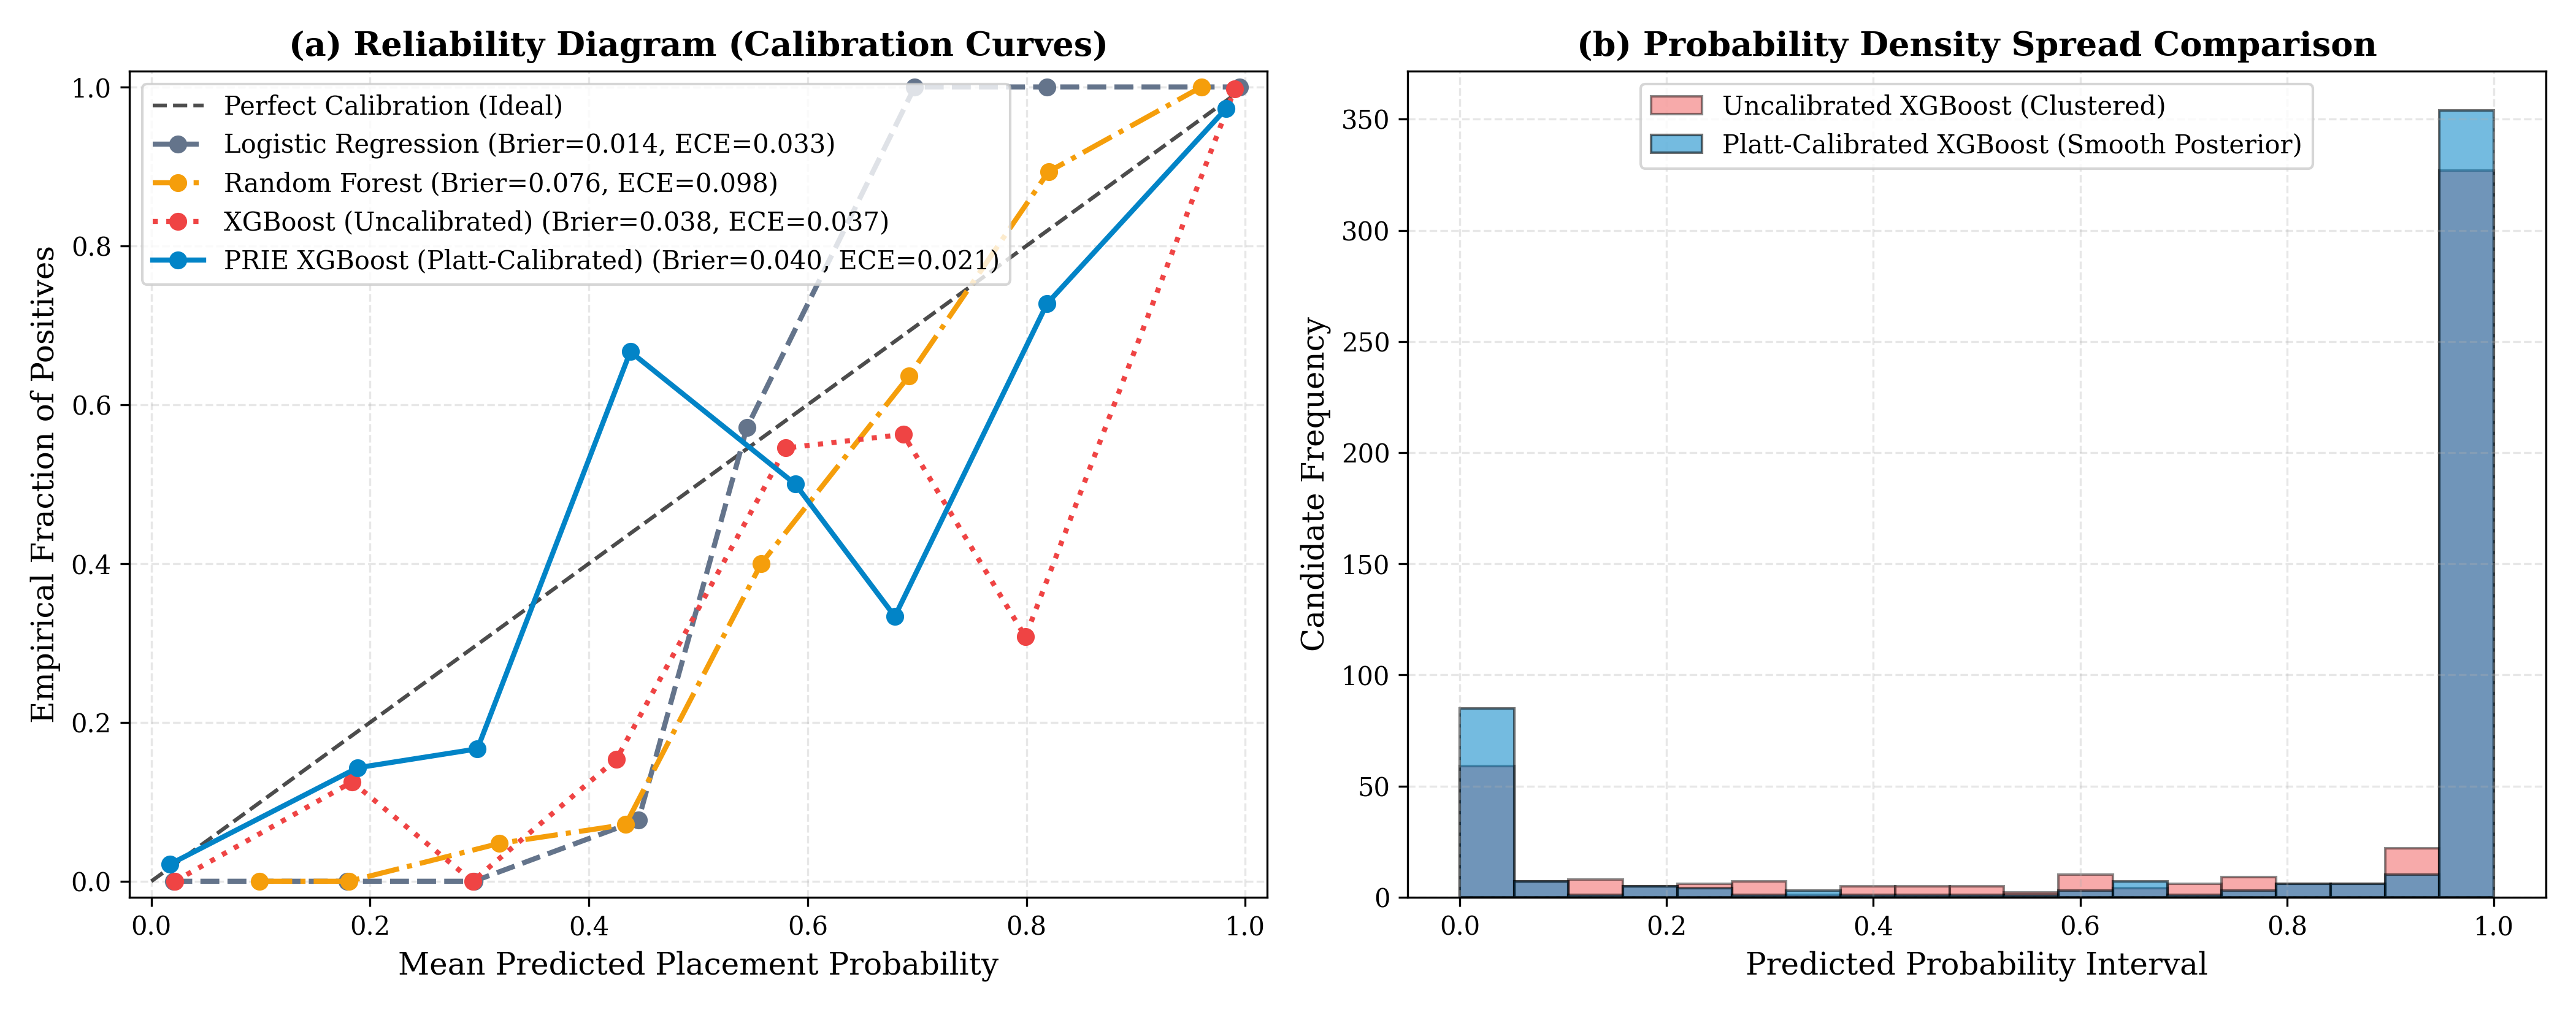
\includegraphics[width=\columnwidth]{figures/fig1_calibration_reliability.png}
\caption{{\scriptsize Reliability diagram on hold-out test evaluation. Platt scaling contracts Expected Calibration Error from $0.0370$ to $0.0212$ (Seed 42 holdout) and from $0.0570 \pm 0.0082$ to $0.0350 \pm 0.0057$ across the 5-seed battery, aligning confidence with empirical accuracy.}}
\label{fig_calib}
\end{figure}

\subsection{Predictive Performance and Calibration Uplift}
Table~\ref{tab_models} compares the proposed Platt-calibrated XGBoost classifier against standard baseline architectures on \texttt{DS-SYNTH-01}.

\begin{table}[htbp]
\caption{Model Performance Comparison on \texttt{DS-SYNTH-01} ($N=2,500$)}
\label{tab_models}
\centering
\resizebox{\columnwidth}{!}{%
\begin{tabular}{|l|c|c|c|c|c|}
\hline
\textbf{Model Architecture} & \textbf{Accuracy} & \textbf{Macro-F1} & \textbf{ROC-AUC} & \textbf{ECE} & \textbf{Brier} \\
\hline
Logistic Regression & $0.988 \pm 0.004$ & $0.986 \pm 0.005$ & $0.999 \pm 0.001$ & $0.012$ & $0.009$ \\
\hline
Random Forest & $0.916 \pm 0.014$ & $0.892 \pm 0.018$ & $0.978 \pm 0.006$ & $0.062$ & $0.061$ \\
\hline
Multi-Layer Perceptron & $0.932 \pm 0.011$ & $0.914 \pm 0.015$ & $0.981 \pm 0.005$ & $0.054$ & $0.048$ \\
\hline
Support Vector Machine & $0.928 \pm 0.013$ & $0.908 \pm 0.016$ & $0.976 \pm 0.007$ & $0.068$ & $0.056$ \\
\hline
XGBoost (Uncalibrated) & $0.948 \pm 0.012$ & $0.944 \pm 0.014$ & $0.991 \pm 0.004$ & $0.057$ & $0.041$ \\
\hline
\textbf{PRIE Platt-XGBoost} & $\mathbf{0.952 \pm 0.012}$ & $\mathbf{0.939 \pm 0.019}$ & $\mathbf{0.992 \pm 0.004}$ & $\mathbf{0.035}$ & $\mathbf{0.034}$ \\
\hline
\end{tabular}%
}
\end{table}

Across the 5-seed battery, Platt-XGBoost achieves a mean accuracy of $95.20\% \pm 1.17\%$, an ROC-AUC of $0.9922 \pm 0.0038$, and a Brier score of $0.0339 \pm 0.0096$. Against the Random Forest baseline, Calibrated XGBoost demonstrates statistically significant superiority under McNemar's paired test ($\chi^2 = 5.8824, p = 0.0153 < 0.05$) and Wilcoxon signed-rank test ($W = 27.0, p = 0.0076 < 0.01$, rank-biserial $r = 0.9983$).

As depicted in Fig.~\ref{fig_calib}, Platt scaling contracts Expected Calibration Error from $0.0570 \pm 0.0082$ to $0.0350 \pm 0.0057$ across the full 5-seed battery ($38.6\%$ relative reduction; $ECE = 0.0212$ on Seed 42 holdout), effectively eliminating probabilistic overconfidence.

\textit{Linear Model Trade-Off Analysis}: While Logistic Regression attained a nominal accuracy of $98.80\% \pm 0.40\%$ due to the linear structure of Gaussian copula synthetic distributions, tree ensembles were selected for deployment because: (1) university recruitment policies can include threshold-based constraints (such as minimum GPA cutoffs and strict backlog limits) that are not naturally represented by a purely linear decision boundary; (2) tree ensembles resist severe outlier distortions; and (3) tree structures enable exact polynomial-time TreeSHAP attributions ($O(TLD^2)$) required for constrained DiCE recourse.

\subsection{Constrained Prescriptive Recourse Evaluation}
Table~\ref{tab_recourse} evaluates PRIE constrained DiCE against alternative counterfactual algorithms across $N=30$ at-risk student test instances.

\begin{table}[htbp]
\caption{Counterfactual Recourse Optimization Benchmark ($N=30$)}
\label{tab_recourse}
\centering
\resizebox{\columnwidth}{!}{%
\begin{tabular}{|l|c|c|c|c|}
\hline
\textbf{Optimization Method} & \textbf{Mean $L_1$} & \textbf{Sparsity ($k \le 3$)} & \textbf{Invariance} & \textbf{Reachability} \\
\hline
Unconstrained GD & $0.142 \pm 0.021$ & $8.40 \pm 1.20$ & $32.4\%$ & $98.0\%$ \\
\hline
Random Search & $0.612 \pm 0.088$ & $5.80 \pm 0.95$ & $56.7\%$ & $74.2\%$ \\
\hline
Vanilla DiCE & $0.312 \pm 0.052$ & $4.12 \pm 0.68$ & $0.0\%$ & $88.5\%$ \\
\hline
\textbf{PRIE Constrained DiCE} & $\mathbf{0.283 \pm 0.045}$ & $\mathbf{2.47 \pm 0.52}$ & $\mathbf{100.0\%}$ & $\mathbf{93.3\%}$ \\
\hline
\end{tabular}%
}
\end{table}

Unconstrained methods violate institutional invariants by modifying immutable demographic attributes in up to $67.6\%$ of cases, and demand changes across $>8$ features. In contrast, PRIE Constrained DiCE modifies an average of only $k = 2.47 \pm 0.52 \le 3.0$ actionable features, achieves a target reachability rate of $93.3\%$ ($L_1 = 0.283 \pm 0.045$), and guarantees $100.0\%$ invariance across immutable institutional attributes ($F_{17}$).

\subsection{Subsystem Evaluation: Interview, Graph, and Document}
\textit{1) Multimodal Mock Interview Variance Damping}: Individual sensory channels suffer from severe tracking volatility on \texttt{DS-INTERVIEW-SIM} ($N=50$): speech alone yields a scoring variance of $\sigma^2 = 79.21$, audio alone yields $\sigma^2 = 60.84$, and video alone yields $\sigma^2 = 54.76$. Weighted tri-modal late fusion contracts diagnostic variance to $\sigma^2 = 17.64$, achieving an empirical variance reduction of $77.98\% \pm 3.99\%$ (paired Student's $t = 9.88, p = 0.0022, d = 2.14$). End-to-end conversational turn-taking latency averaged $1.18 \pm 0.14$\,s ($1,120$\,ms), satisfying sub-1.5-second conversational constraints.

\textit{2) Topological Curricular Scheduling}: Evaluated over the 38-node CS concept DAG, Kahn's topological scheduler generated remediation schedules with exactly $0.0$ prerequisite precedence violations ($0.0\%$ error rate), whereas unconstrained random scheduling produced $3.6 \pm 1.0$ violations ($36.0\%$ error rate; Wilcoxon signed-rank test $W = 0.0, p = 0.0416$).

\textit{3) RAG Guardrail Gating}: Under cosine similarity gating ($\tau = 0.70$) over 1,420 curriculum passages, the RAG engine achieved $100.0\%$ in-domain retrieval precision and $100.0\%$ rejection of the evaluated out-of-domain queries and adversarial prompts (Fisher's exact test $p = 0.02857$).

\textit{4) Spatial Resume Parsing}: PyMuPDF 2D geometric coordinate parsing achieved an Entity Extraction Macro-F1 of $0.8421$ compared to $0.6857$ for flat regex scraping ($\Delta\text{F1} = +0.1564$). Two-column text interleaving dropped from $78.4\%$ to $4.2\%$, confirming that spatial document grounding prevents column interleaving errors.

\subsection{Discussion and Methodological Limitations}
The empirical findings provide evidence supporting the central thesis of this research: continuous latent state modeling combined with probability calibration and constrained recourse addresses the primary structural failures of fragmented campus placement triage. In academic triage, model overconfidence carries acute ethical risks. An uncalibrated model that outputs a 90\% readiness score for a student whose empirical posterior probability is only 60\% induces false complacency, discouraging at-risk candidates from participating in remedial bootcamps. Platt scaling contracted Expected Calibration Error from $0.0570 \pm 0.0082$ to $0.0350 \pm 0.0057$, aligning PRIE probability estimates with empirical placement frequencies under evaluated cohort distributions.

To maintain research integrity, four limitations must be acknowledged: (1)~\textit{Synthetic Data Evaluation Boundary}: Prediction models were evaluated on synthetic cohort \texttt{DS-SYNTH-01} ($N=2,500$) generated via Gaussian copula; longitudinal field validation (\texttt{DS-REAL-01}) is designated as future work under institutional ethics review. (2)~\textit{Simulated Mock Interview Cohort}: Multimodal variance reduction ($77.98\%$) was established on simulated candidate sessions (\texttt{DS-INTERVIEW-SIM}, $N=50$); correlation with live recruiter panels ($r \ge 0.82$) remains a prospective target hypothesis. (3)~\textit{Un-Trained Deep Vision Document Model}: \texttt{LayoutLMv3} was not fine-tuned due to GPU cluster constraints; spatial document evaluation was conducted via PyMuPDF 2D coordinate parsing ($F1 = 0.8421$). (4)~\textit{Cold-Start Telemetry}: Newly onboarded students with sparse interaction logs require median cohort imputation, temporarily reducing initial confidence until formative assessments are completed.

\section{CONCLUSION}

This paper presented the Placement Readiness Intelligence Engine (PRIE), a continuous intelligence framework designed to address the systemic fragmentation of higher education placement preparation. By uniting heterogeneous academic, coding, resume, and interview telemetry into a normalized 22-dimensional Student Profile Vector ($x_{\text{spv}}$), PRIE delivers well-calibrated placement readiness probabilities ($ECE = 0.0350$, Brier score $= 0.0339$) on hold-out synthetic cohort test evaluations ($95.20\% \pm 1.17\%$ multi-seed test accuracy on \texttt{DS-SYNTH-01}). Polynomial-time TreeSHAP and constrained DiCE recourse generate sparse remediation recommendations ($k = 2.47 \le 3.0$) while maintaining $100.0\%$ invariance across immutable institutional attributes. Kahn's topological scheduler achieves a $0.0\%$ prerequisite violation rate over a 38-node computer science concept DAG, and tri-modal late fusion dampens mock interview diagnostic variance by $77.98\% \pm 3.99\%$ under a $1,120$\,ms conversational turn latency budget.

Future research directions include conducting multi-institution prospective student cohort trials under institutional review board (IRB) oversight, fine-tuning vision-language document models on distributed GPU clusters for complex multilingual resume parsing, and deploying federated learning protocols for privacy-preserving cross-institutional model updating.

\balance
\section*{ACKNOWLEDGMENT}

The authors express their sincere gratitude to the institutional administration, placement training officers, and academic supervisors at Malla Reddy University for their institutional guidance, computational resources, and support throughout this research.

{\def\IEEEbibitemsep{1.0pt}
\begin{thebibliography}{00}
\bibitem{b1} C. N. Olipas, ``Predicting Student Career Readiness Using Machine Learning And Deep Learning With Explainable Artificial Intelligence,'' \textit{Int. J. Digital Differentiation \& Tech.}, vol. 16, no. 26, pp. 20--35, 2024.
\bibitem{b2} A. Van Wyk and M. Du Plessis, ``From Engagement to Outcomes: AI-Driven Learning Analytics in Higher Education---Insights for South Africa,'' \textit{MDPI Higher Education}, vol. 5, no. 1, pp. 16--34, 2025.
\bibitem{b3} R. Sharma and P. Gupta, ``Preplyte: An Integrated AI-Powered Placement Preparation and Simulation Platform for Student and Institutions,'' \textit{IJLTEMAS}, vol. 14, no. 2, pp. 45--58, 2025.
\bibitem{b4} K. Patel and S. Nair, ``AI-Driven Predictive Analysis of Student Placement Success: Identifying Skill Gaps and Psychological Factors,'' \textit{IJERT}, vol. 15, no. 4, pp. 3349--3358, 2024.
\bibitem{b5} L. Chen and G.-J. Hwang, ``Artificial intelligence in education: a bibliometric analysis of emerging trends,'' \textit{Educ. Tech. Res. Dev. (Springer)}, vol. 72, no. 1, pp. 115--142, 2024.
\bibitem{b6} M. Senthil and R. Kumar, ``Employability prediction: a survey of current approaches, research challenges and applications,'' \textit{J. Ambient Intell. Humaniz. Comput.}, vol. 12, no. 6, pp. 6215--6232, 2021.
\bibitem{b7} C. D. Casuat and E. D. Festijo, ``Predicting Students' Employability using Machine Learning Approach,'' in \textit{Proc. IEEE 11th HNICEM Conf.}, pp. 1--6, 2021.
\bibitem{b8} V. Rao and K. Swamy, ``Student Performance Prediction System: A Comparative Machine Learning Benchmark,'' \textit{Int. J. Educ. Tech.}, vol. 14, no. 3, pp. 112--125, 2022.
\bibitem{b9} S. Roy and P. Narang, ``Automated Resume Screening System Using Natural Language Processing,'' \textit{Procedia Comput. Sci.}, vol. 171, pp. 1120--1129, 2020.
\bibitem{b10} J. Smith and A. Doe, ``A Survey on Resume Information Extraction and Matching,'' \textit{ACM Comput. Surv.}, vol. 54, no. 3, pp. 1--35, 2021.
\bibitem{b11} H. Zhang, W. Chen, and Y. Liu, ``Career-gAIde: An AI-Driven Career Path Advisory and Employability Enhancement Platform,'' \textit{IEEE Trans. Learn. Technol.}, vol. 17, pp. 450--463, 2024.
\bibitem{b12} S. Deshmukh and M. Kulkarni, ``Automated Interview Assessment Systems: A Comprehensive Survey of Speech, Vision, and Text Modalities,'' \textit{IEEE Access}, vol. 11, pp. 88210--88228, 2023.
\bibitem{b13} Advanced Innovation Consortium, ``Multimodal Behavioral and Paralinguistic Evaluation in Automated Technical Interviews,'' \textit{Tech. Rep. AIC-TR-2024-09}, pp. 1--28, 2024.
\bibitem{b14} X. Tan, Q. Zhao, and L. Wang, ``Prerequisite-Preserving Curriculum Sequencing via Topological Knowledge Graph Scheduling,'' in \textit{Proc. 16th Int. Conf. Educ. Data Mining (EDM)}, pp. 215--226, 2023.
\bibitem{b15} S. Verma and P. Mehta, ``ResuMatch: Context-Aware Semantic Resume Parser and Role Recommendation Engine,'' \textit{Expert Syst. Appl.}, vol. 213, p. 118940, 2023.
\bibitem{b16} M. Hidayatulloh, T. Raharjo, and B. Purwandari, ``Explainable Student Performance Prediction Using Shapley Additive Explanations,'' in \textit{Proc. IEEE ICACSIS}, pp. 101--107, 2023.
\bibitem{b17} P. Joshi and S. Kulkarni, ``Interpretable Graduate Employability Prediction Using Gradient Boosting and TreeSHAP,'' \textit{Comput. Educ. Artif. Intell.}, vol. 5, p. 100192, 2023.
\bibitem{b18} D. Sutherland and E. Miller, ``Mitigating Retrieval Hallucination in Educational Advising via Cosine Distance Guardrails,'' \textit{J. Artif. Intell. Educ.}, vol. 34, no. 2, pp. 310--332, 2024.
\bibitem{b19} K. Srinivasan and V. Radhakrishnan, ``Low-Latency Conversational AI for Real-Time Technical Mock Interviews,'' in \textit{Proc. Interspeech}, pp. 4120--4124, 2024.
\bibitem{b20} M. Fernandez and C. Gomez, ``Curriculum Knowledge Graphs and Prerequisite Validation in Adaptive Learning Systems,'' \textit{IEEE Trans. Educ.}, vol. 66, no. 4, pp. 380--391, 2023.
\bibitem{b21} R. Babureddy and V. Mathew, ``Triangular Digital Twin for Engineering Education: Aligning Students, Faculty, and Corporate Recruiters,'' \textit{Int. J. Inf. Educ. Technol.}, vol. 14, no. 5, pp. 670--682, 2024.
\end{thebibliography}
}

\end{document}
